% concatenated from comparing_walks.tex
\documentclass[11pt,a4paper]{article}
\usepackage{amssymb,comment,amsmath,amsthm}
\usepackage{graphicx}
\usepackage{color}
\usepackage{titling,titlesec}
\usepackage{url}
\usepackage{amsthm,lipsum}
\usepackage{geometry}
\usepackage{tikz}
\usepackage{hyperref}
\titleformat{\subsection}[runin]
{\normalfont\bfseries}{}{0em}{}[.]
\newcounter{foo}
\newcommand{\red}[1]{\textcolor{red}{#1}}
\newfont{\blb}{msbm10 scaled\magstep1}
\newfont{\comp}{cmr12 scaled\magstep1}
\newfont{\compb}{cmr10 scaled\magstep2}
\newfont{\sbb}{cmssbx10 scaled\magstep3}
\newfont{\sbbb}{cmssbx10 scaled\magstep5}
\newfont{\sbs}{cmssbx10 scaled\magstep1}
\newtheorem{theorem}{Theorem}
\newtheorem{lemma}[subsection]{Lemma}
\newtheorem{claim}[subsection]{Claim}
\newtheorem{cl}[section]{Claim}
\newtheorem{corollary}[subsection]{Corollary}
\newtheorem{proposition}{Proposition}
\newtheorem{definition}[foo]{Definition}
\newtheorem{conjecture}{Conjecture}
\newtheorem{question}{Question}
\newtheorem{example}{Example}
\def\cC{\mathcal C}
\newcommand{\cev}[1]{\reflectbox{\ensuremath{\vec{\reflectbox{\ensuremath{#1}}}}}}
\newcommand{\bs}{{\scriptstyle \blacksquare}}
\newcommand{\RR}{{\mathbb R}}
\newcommand{\NN}{{\mathbb N}}
\newcommand{\Zd}{{\mathbb Z}^d}
\newcommand{\Ed}{{\mathrm{E}}^d}
\newcommand{\PP}{{\mathbb P}}
\newcommand{\EE}{{\mathrm{E}}}
\newcommand{\eps}{\varepsilon}
\newcommand{\im}{\mathrm{Im}}
\newcommand{\mon}{\mathrm{Inj}}
\newcommand{\Hom}{\mathrm{Hom}}
\newcommand{\vep}{\varepsilon}
\newcommand{\Supp}{\mathrm{Supp}}
\allowdisplaybreaks
%\usepackage{hyperref}
%\hypersetup{colorlinks = true, linkcolor=black, citecolor = {black}, urlcolor = black}
\setlength{\parindent}{0pt} \oddsidemargin -0.1in \evensidemargin
-0.1in \topmargin -0.4in \textheight 9in \textwidth 6.3in
\renewcommand{\baselinestretch}{1.02}
\geometry{margin = 1in}
\title{A General Inequality for Walks in Graphs}
\author{
Chase Wilson\thanks{Department of Mathematics, University of California, San Diego, CA, 92093-0112 USA. E-mail: c7wilson@ucsd.edu}}
%%%%%%%%%%%%%%%%%%%%%%%%%%%%%%%%%%%%%%%%%%%%%%%%%%%%%%%%%%%%%%%%%%%%%%%%
\begin{document}
\date{}
\setlength{\droptitle}{-2.5cm}
\maketitle
\vspace{-0.5in}

\begin{abstract}
Let $G$ be a graph and $w_k(G)$ denote the number of walks in $G$ of length $k$. For sequences $a_1, \cdots, a_n$ and $b_1, \cdots, b_n$ of non-negative integers such that $a_1 + \cdots + a_n = b_1 + \cdots + b_n$, we determine a simple necessary and sufficient condition on $a_1, \cdots, a_n, b_1, \cdots, b_n$ for the inequality
\[
w_{a_1}(G) \cdots w_{a_n}(G) \geq w_{b_1}(G) \cdots w_{b_n}(G)
\]
to hold for any graph $G$. 
\end{abstract}
\begin{section}{Introduction}
Let $G$ be a graph. A \textit{walk} on $G$ is a sequence of vertices $v_1, \cdots, v_n$ such that $\{v_i, v_{i + 1} \} \in E(G)$ for all $1 \leq i \leq n - 1$. We denote by $w_n(G)$ the number of walks on $G$ of length of $n$. For our purposes, the length of a walk is the number of edges it contains.

\medskip

The study of counting walks in graphs has a long history. In 1965, Blakely and Roy \cite{BlR} proved that $w_n(G) w_0(G)^{n - 1} \geq w_1(G)^n$ for all $n \geq 1$. Erd\H{o}s and Simonovits \cite{ES} proved that $w_k(G)^t \geq w_t(G)^k w_0(G)^{t - k}$ when both $k$ and $t$ are even and $k \geq t$. They cojectured that the same result holds when both $k$ and $t$ are odd. This was recently proved by Saglam, and later Raymond and Blekherman \cite{BR} gave a substantially simpler proof. Further inequalities of this type have also been studied. Lagarius \cite{LM} showed that $w_{2a + b}(G) w_b(G) \leq w_0(G) w_{2a + 2b}(G)$ Dress and Gutman \cite{DG} showed that $w_{a + b}(G)^2 \leq w_{2a}(G) w_{2b}(G)$. Hemecke, Kosub, et al. \cite{HK} generalized these two results by proving the so called sandwhich theorem which states $w_{2a + c} (G)w_{2(a + b) + c}(G) \leq w_{2a}(G) w_{2(a + b + c)}(G)$. They also proved $w_{2 \ell + p}(G)^k \leq w_{2 \ell}(G)^{k - 1} w_{2 \ell + pk}(G)$. Raymond and Blekherman \cite{BR2}, unknown to us during our research, used Tropical Geometry to give a list of inequalties and show that any true inequality of the above type can be deduced from one on their list.

\medskip

We prove the following.

\begin{definition} Let $a_1, \cdots, a_n, b_1, \cdots, b_n$ be non-negative integers such that $a_1 + \cdots + a_n = b_1 + \cdots + b_n$. Let $b^o_1 \geq \cdots \geq b^o_q$ be the odd integers (counted with multiplicity) among $b_1, \cdots, b_n$ and $b^e_1 \geq \cdots \geq b^e_{n - q}$ be the even integers (counted with multiplicity) among $b_1, \cdots, b_n$. We say that $(a_1, \cdots, a_n)$ \textit{majorizes} $(b_1, \cdots, b_n)$ \textit{with parity} if the following holds. For all $i \in [0, q]$ and $j \in [0, n - q]$ there are at least $(i + j)$ elements from $a_1, \cdots, a_n$ that are either even or greater than or equal to $b^o_i$ and, letting $a'_1, \cdots, a'_{i + j}$ be the $(i + j)$ largest such elements (counted with mulitplicity),
\[
\left ( \sum_{k = 1}^i b^o_k \right ) + \left ( \sum_{k = 1}^j b^e_k \right ) \leq \sum_{k = 1}^{i + j} a'_{k}
\]
\end{definition}
\begin{theorem} \label{main}
Let $a_1, \cdots, a_n, b_1, \cdots, b_n$ be non-negative integers such that $a_1 +\cdots + a_n = b_1 +\cdots + b_n$. Then the inequality $w_{a_1}(G) \cdots w_{a_n}(G) \geq w_{b_1}(G) \cdots w_{b_n}(G)$ holds for any graph $G$ iff $(a_1, \cdots, a_n)$ majorizes $(b_1, \cdots, b_n)$ with parity.
\end{theorem}
The main advantages this has over the Raymond Blekherman \cite{BR2} result, is that first, our proof is significantly shorter and purely combinatorial, and second, given a proposed inequality, our result gives a simple way to check if it is true or not. In order to get the concise description of true inequalities, we do sacrifice a slight bit generality compared to the Raymond Blekherman result as their generating inequalities are not restricted to ones where $a_1 + \cdots + a_n = b_1 + \cdots + b_n$. We also note that translating from a generating to set of inequalities to our consise description is non-trivial. Indeed, our approach also starts by giving a (different) list of generating inequalities but the bulk of this paper is spent showing that it is possible to derive an inequality of the form $w_{a_1} \cdots w_{a_n} \geq w_{b_1} \cdots w_{b_n}$ from our generating set of inequalities precisely when $a_1, \cdots, a_n$ majorizes $b_1, \cdots, b_n$ with parity.

\medskip

Theorem \ref{main} holds for mult-graphs as well as graphs. By considering the adjacency matrix of $G$, and using rational approximation we can translate this into the language of symmetric matrices.
\begin{corollary} Let $a_1, \cdots, a_n, b_1, \cdots, b_n$ be non-negative integers such that $a_1 + \cdots + a_n = b_1 +\cdots + b_n$. Then
\[
\prod_{i = 1}^n \langle A^{a_i} \boldsymbol{1}, \boldsymbol{1} \rangle \geq \prod_{i = 1}^n \langle A^{b_i} \boldsymbol{1}, \boldsymbol{1} \rangle
\]
holds for any symmetric matrix $A$ with non-negative entries iff $(a_1, \cdots, a_n)$ majorizes $(b_1, \cdots, b_n)$ with parity. 
\end{corollary}

\begin{subsection}{Organization} In Section \ref{sec2}, we use entropy techniques inspired by Raymond and Blekherman \cite{BR} to prove the if direction in Theorem \ref{main} in the special case that $b_1 = b_2 = \cdots = b_n$. In Section \ref{sec3}, we prove the full if direction of Theorem \ref{main} by averaging many instances of the special case where $b_1 = b_2 = \cdots = b_n$. In Section \ref{sec4}, we prove the only if direction of Theorem \ref{main} by, given a pair of sequences $(a_1, \cdots, a_n)$, $(b_1, \cdots, b_n)$ for which $(a_1, \cdots, a_n)$ does not majorize $(b_1, \cdots, b_n)$ with parity, constructing a graph $G$ in which $w_{a_1}(G) \cdots w_{a_n}(G) < w_{b_1}(G) \cdots w_{b_n}(G)$. 

\end{subsection}
\begin{section}{Notation and Entropy} \label{sec2}

\begin{subsection}{Notation}
For a matrix $M$, we let $M_i$ denote the $i$th row of $M$. We let $\bf{1}$ be the all $1$ vector. For vectors $v, w$, we say $v \leq w$ if $v$ is less than or equal to $w$ pointwise. For a graph $G$ and non-negative integer $k$, we let $w_k(G)$ denote the number of walks of length $k$ in $G$. When the graph $G$ is obvious from context we just write $w_k$.For a vector $v$, we let $\dim(v)$ be the dimension of $v$. 

\medskip

We say that $f(x) \ll g(x)$ if $f = o(g)$. 
\end{subsection}
\begin{subsection}{Entropy} We use entropy in section \ref{sec_p1}. Let us recall the basics of entropy.
If $S$ is a finite set and $X, Y$ are $S$-valued random variable, then the {\em entropy of $X$} is given by
\[
	H[X] = -\sum_{y \in \im(X)} P(X = y) \log ( P(X = y) )
\]
and the {\em conditional entropy} $H[X | Y]$ is given by
\[
	H[X | Y] = E_{y \sim Y} [ H[(X | Y = y)]]
\]
The two main facts of entropy that we will make use of are as follows:
\begin{proposition}
Let $X,X_1,X_2,\dots,X_k$ be random variables where $X$ has values in $S$ and $X_i$ has values in $S_i$ for $1 \leq i \leq k$.
\begin{center}
\begin{tabular}{lp{5in}}
$1$. & {\rm [Uniform bound]} $H[X] \leq \log( |\im(X)| )$ with equality iff $X$ has uniform distribution.\\
$2$. & {\rm [The Chain Rule]} $(X_1,X_2, \cdots, X_k)$ is an $S_1 \times \cdots \times S_k$ random variable and $H[X_1, \cdots, X_k] = H[X_1] + H[X_2 | X_1] + \cdots + H[X_k | X_1, \cdots, X_{k - 1} ]$.
\end{tabular}
\end{center}
\end{proposition}
\end{subsection}
\end{section}
\end{section}

\begin{section}{A Simpler Inequality} \label{sec_p1}
In this section we prove the following Lemma which will be used to prove Theorem \ref{main}..
\begin{lemma} \label{simple} Let $a_1, \cdots, a_n, b$ be integers such that $a_1 + \cdots + a_n = bn$, then
\[
w_{a_1} \cdots w_{a_n} \geq w_b^n
\]
for any graph $G$ if either
\begin{itemize}
\item $b$ is odd and $a_i$ is even whenever $a_i < b$.
\item $b$ is even and $a_i$ is even for all $i$.
\end{itemize}
\end{lemma}
Note this is precisely the if direction in Theorem \ref{main} in the special case where $b_1 = \cdots = b_n$. We will focus on proving this inequality when the first bullet holds since the second will follow from the exact same argument.

\begin{definition} We say walks $p_1, \cdots p_n$ in a graph $G$ can be arranged into the walks $q_1,\cdots, q_k$ if for every ordered pair $(u, v)$ of adjacent vertices in $V(G)$, $(u, v)$ is crossed (with this orientation) the same number of times in $p_1, \cdots, p_n$ as in $q_1, \cdots, q_k$.
\end{definition}

In order to use entropy, we aim to show that given a walk $W$ of length $b$, there exists $n$ walks $\rho_1, \cdots, \rho_n$ of length $a_1,\cdots, a_n$ that can be arranged into $n$ walks $\gamma_1, \cdots, \gamma_n$ each of length $b$ such that for all $i$, $\gamma_i$ is either $W$ or the the reverse of $W$ and the start and endpoint of $\rho_i$ are endpoints of $W$.


\[
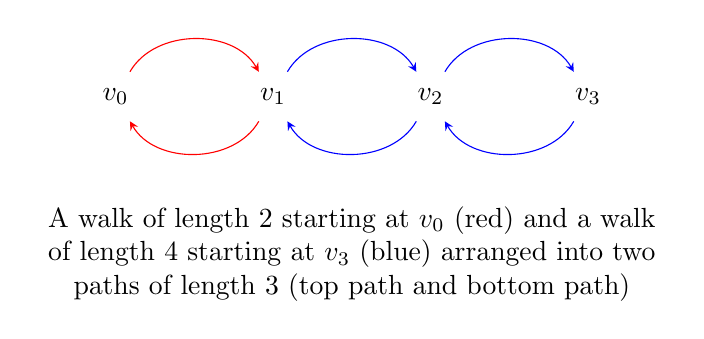
\begin{tikzpicture}
\tikzset{
  every arrow/.style={line width=1.5pt},
  >=stealth
}
\node[circle] (A) at (0, 0){$v_0$};
\node[ circle] (B) at (2, 0) {$v_1$};
\node[ circle] (C) at (4, 0) {$v_2$};
\node[ circle] (D) at (6, 0) {$v_3$};

\node[align = flush center, text width = 8cm] (Label) at (3, -2)
{
A walk of length $2$ starting at $v_0$ (red) and a walk of length $4$ starting at $v_3$ (blue) arranged into two paths of length $3$ (top path and bottom path)
};

\path[red, ->]  (A) edge[out = 60, in = 120] (B);
\path[red, ->]  (B) edge[out = -120, in = -60] (A);

\path[blue, ->]  (D) edge[out = -120, in = -60] (C);
\path[blue, ->]  (C) edge[out = -120, in = -60] (B);

\path[blue, ->]  (B) edge[out = 60, in = 120] (C);
\path[blue, ->]  (C) edge[out = 60, in = 120] (D);

\end{tikzpicture}
\]
\begin{lemma}\label{decompose_lemma} Let $P_b = (0, \cdots, b)$ be the path of length $b$ and let $q_1, \cdots, q_{r}$ be paths in $P_b$ of the form $q_i = (u_i, w_i, u_i)$ for some vertices $w_i, u_i \in P_b$. Then if $s, t$ are positive integers such that $s + t = b + r$, there exists paths $p, \gamma$ such that
\begin{itemize}
\item $p$ has length $2s$, $\gamma$ has length $2t$.
\item $p$ and $\gamma$ can be arranged into $(0, \cdots, b), (b, \cdots, 0), q_1, \cdots, q_r$.
\item $p$ starts and ends on $0$ and $\gamma$ starts and ends on $b$
\end{itemize}
\end{lemma}
\begin{proof}
Let us assume that $q_1, \cdots, q_r$ are sorted by their start points so $u_1 \leq u_2 \leq \cdots \leq u_r$. We will start by constructing $p = (p_{0}, \cdots, p_{ 2s} )$ greedily. Conceptually, this means we walk along $P_b$, backtraking by $1$ to cover any $q_i$ we can, and then moving forward and finally returning to $0$ when we are out of length. Formally, we initiate $j = 1$ and do the following inductively: Suppose we have constructed $(p_{0}, \cdots, p_{ i - 1} )$. If $p_{ i - 1} = 2s - (i - 1)$, then let $(p_{i}, \cdots, p_{ 2s} ) = (2s - (i - 1) - 1, \cdots, 0)$ and let $M = 2s - (i - 1)$. If that is not the case and $p_{ i - 1} = u_j$, then let $(p_{i}, p_{ i + 1}) = (v_j, u_j)$ and increment $j$ by $1$. Otherwise let $p_{ i} = p_{ i - 1} + 1$.

\medskip

If $j_1$ is the maximum $j$ gets incremented to, then we can arrange $p$ into $q_1, \cdots, q_{j_1 - 1}, (0,\cdots, M_1 - 1, M_1, M_1 - 1, \cdots, 0)$ when $M_1$ is the maximum $p_i$ is at the beginning of one of the steps.

\medskip

We then do the same greedy strategy to construct $\gamma$ but in reverse. We initiate $j = r$ and again do the following inductively: Suppose we have constructed $(\gamma_{0}, \cdots, \gamma_{ i - 1} )$. If $\gamma_{ i - 1} = b - ( 2s - (i - 1))$, then let $(\gamma_{i}, \cdots, \gamma_{ 2s} ) = ( b- (2s - (i - 1)) + 1, \cdots, b)$. Otherwise if $\gamma_{ i - 1} = u_j$, then let $(\gamma_{i}, \gamma_{ i + 1}) = (v_j, u_j)$ and decrement $j$ by $1$. Otherwise let $\gamma_{ i} = \gamma_{ i - 1} - 1$.

\medskip

If $j_2$ is the minimum $j$ gets decremented to, we can arrange $\gamma$ into $q_{j_2 + 1}, \cdots, q_r, (b, \cdots, M_2 + 1, M_2, M_2 + 1, \cdots b)$.

\medskip

Since $(0, \cdots,M - 1, M, M - 1, \cdots, 0), (b, \cdots, M + 1, M, M + 1, \cdots b)$ can be arranged into $(0, \cdots, b), (b, \cdots, 0)$, it suffices to show that $M_1 = M_2$ and $j_1 = j_2 + 1$. We have
\[
b + r = s + t = M_1 + (b - M_2) + (j_1 - 1) + (r - j_2)
\]
which implies
\[
(M_1 - M_2) = (j_2 + 1 - j_1)
\]
We also have $u_{j_1 - 1} \leq M_1 \leq u_{j_1}$ and $u_{j_2 + 1} \leq M_2 \leq u_{j_2}$ (Here we set $u_0 = 0$ and $u_{r + 1} = b$). Since $u_i$ is a non-decreasing sequence, this implies that $M_1 = M_2$ and $j_2 + 1 = j_1$
\end{proof}
\begin{lemma} \label{lemma_2} Let $b$ be non-negative integer $a_1, \cdots, a_n, r, b$ are non-negative integers such that an even number of the $a_i$ are even, all $a_i$ with $a_i < b$ are even and $a_1 + \cdots + a_n + 2r = n b$. Then there exists paths $p_1, \cdots, p_n$, and $q_1, \cdots, q_r$ in $P_b = (0, \cdots, b)$ such that
\begin{enumerate}
\item $p_i$ has length $a_i$ for all $1 \leq i \leq n$.
\item $p_i$ starts and ends at an endpoint of $P_b$ for all $1 \leq i \leq n$
\item $q_i$ has length $2$ for all $i$
\item $q_i$ starts and ends at the same vertex for all $i$.
\item $p_1, \cdots, p_n, q_1, \cdots,q_r$ can be arranged into $P'_1, \cdots, P'_n$ where, for all $1 \leq i \leq n$, $P'_i$ is is either $(0,\cdots, b)$ or $(b, \cdots, 0)$.
\end{enumerate}
\end{lemma}
\begin{proof} We use induction. First suppose one of the $a_i$ is odd. Without loss of generality assume it is $a_n$. Then let us apply the inductive hypothesis with input $a_1, \cdots, a_{n - 1}, r + (a_n - b)/2, b$ to get paths $p_1, \cdots, p_{n - 1}$, $q_1, \cdots, q_{r + (a_n - b)/2}$. Let $p_n$ be a path in $P_b$ that can be arranged into $P_b, q_1, \cdots, q_{ (a_n - b)/2}$. Then it is not difficult to see that the paths $p_1, \cdots, p_n$ and $q_{(a_n - b)/2}, \cdots, q_{r + (a_n - b)/2}$ satisfy $1$-$5$.

\medskip

Now suppose that all the $a_i$ are even. Since $a_1 + \cdots + a_n + 2r = n b$, there must exist indices $1 \leq i < j \leq n$ such that $2 (a_i + a_j + r) \geq 2b$. Without loss of generality assume $i = n - 1$, $j = n$. Let us apply induction with $a_1, \cdots a_{n - 2}, a_i + a_j + r - b$. Then we get paths $p_1, \cdots, p_{n - 2}$, and $q_1, \cdots, q_{a_i + a_j + r - b}$. If $a_i + a_j \geq 2b$, then by lemma \ref{decompose_lemma}, we can let $p_{n- 1}$ be a path that starts and ends at $0$, $p_{n}$ be a path that starts and ends at $b$ and $p_{n - 1}, p_n$ can be arranged into $(0, \cdots, b)$, $(b, \cdots, 0)$ and $q_{r + 1}, \cdots, q_{ (a_i + a_j - 2b)/2 + r }$. In this case the paths $p_1, \cdots, p_n$ and $q_1, \cdots, q_r$ will satisfy $1$-$5$. On the other hand if $a_i + a_j < 2b$, then we can let
\[
p_{n - 1} = (0, \cdots, a_{n - 1}/2, \cdots, 0)
\]
and
\[
p_n = (b, \cdots, b - a_n/2, \cdots, b )
\]
And for $1 \leq i \leq (2b - a_{n - 1} - a_n)/2$, we let
\[
q_{i + r + (a_{n - 1} + a_n - 2b)/2 } = ( a_{n - 1} + i - 1, a_{n - 1} + i, a_{n - 1} + i - 1)
\]
In this case it is clear that $p_1, \cdots, p_n$ and $q_1, \cdots, q_{ r}$ will satisfy $1$-$5$.
\end{proof}

\begin{proof}[Proof of Lemma \ref{simple} ]
We will assume that an even number of the $a_i$ are even as otherwise we can show $w_{a_1}^2 \cdots w_{a_n}^2 \geq w_b^{2n}$ and take the square root of both sides. By Lemma \ref{lemma_2}, there exists paths $p_1, \cdots, p_n$ in $P_b$ of lengths $a_1, \cdots, a_n$, each starting at an endpoint of $P_b$, that can be arranged into $P'_1, \cdots , P'_m, P''_1, \cdots, P''_{n - m}$ such that $P'_i$ is a copy of $P_b$ and $P''_i$ is a copy of $P_b$ reversed for all $i$. Let $\phi_i$ be the map $P_{a_i} \rightarrow P_b$ such defined by
\[
\phi_i ( P_{a_i} (k) ) = p_i (k)
\]
Let us consider the uniform distribution $X = (X_0, \cdots, X_n)$ on walks of length $b$ in $G$. We note that for all $1 \leq i\leq n$, the distribution of $(X_{i +1}, \cdots, X_n)$ given $(X_1, \cdots, X_{i} )$ is the uniform distribution over walks of length $(n - i)$ starting at $X_i$. So $(X_{i +1}, \cdots, X_n)$ is conditionally independent to $(X_1, \cdots, X_{i - 1})$ given $X_i$. Therefore $H[ X_{i + 1} | X_i, \cdots, X_1 ] = H[X_{i + 1} | X_i ]$. Let $\theta^i_k$ be the unique integer such that $p_i(k) = P_b( \theta^i_k)$. Let $Y^i$ be the pullback of $X$ by $\phi_i$. In other words $Y^i$ is the distribution given by
\[
P \left ( (Y^i = (y_0, \cdots, y_{a_i} ) \right ) = P( X_{\theta^i_0} = y_0) \prod_{k = 1}^{a_i} P(X_{\theta^i_k} = y_k | X_{\theta^i_{k - 1}} = y_{k - 1} )
\]
By conditional independence of $X$, we have $P( Y^i_k = y_1) = P(X_{\theta^i_k} = y_1)$ and $P( (Y^i_k, Y^i_{k - 1} ) = (y_1, y_2) ) = P( (X_{\theta^i_k}, X_{\theta^i_{k - 1}}) = (y_1, y_2) )$ for all $k$ and $y_1, y_2 \in V(P_b)$. Therefore by the chain rule,
\begin{align*}
H[Y^i] &= H[Y^i_0] + \sum_{k = 1}^{a_i} H[Y^i_k | Y^i_0, \cdots, Y^i_{k - 1} ]\\
& = H[X_{\theta^i_0}] + \sum_{k = 1}^{a_i} \sum_{v \in P_b} P(X_{\theta^i_{k - 1}} = v) H[ X_{\theta^i_k} | X_{\theta^i_{k - 1}} = v ]\\
&= H[ X_{ \theta^i_0} ] + \sum_{k = 1}^{a_i} H [ X_{ \theta^i_k } | X_{ \theta^i_{k - 1}} ]
\end{align*}
Let $s$ be the number of $i$ such that $p_i(0) = P_b(0)$. Then $n - s$ is the number of $i$ such that $p_i(0) = P_b(b)$. Since paths are symmetric and $X$ is the uniform distribution, we note that $X_0$ has the same distribution as $X_b$. Using this we obtain,
\begin{align*}
\sum_{i = 1}^n \log (w_{a_i}) & \geq \sum_{i = 1}^n H[Y^i] \\
& = s H[X_0] + (n - s) H[X_b] + m \left ( \sum_{i = 1}^b H[X_i | X_{i - 1} ] \right ) + (n - m) \left ( \sum_{i = 1}^b H[X_{b - i} | X_{b - i + 1} ] \right ) \\
& = m \left ( H[X_0] + \sum_{i = 1}^b H[X_i | X_{i - 1} ] \right ) + (n - m) \left ( H[X_b] + \sum_{i = 1}^b H[X_{b - i} | X_{b - i + 1} ] \right ) \\
& = m H(X_0, \cdots, X_b) + (n - m) H(X_b, \cdots, X_0)\\
& = n \log w_b
\end{align*}
Taking exponents we obtain $ w_{a_1}\cdots w_{a_n} \geq w_{b_k}^n$.
\end{proof}



\end{section}




\begin{section}{An Averaging Argument} \label{sec3}
In this section we prove Theorem \ref{main} by averaging instances of Lemma \ref{simple}. That is we aim to prove our main inequality of the form $w_{a_1} \cdots w_{a_n} \geq w_{b_1} \cdots w_{b_k}$ by multiplying together instances of Lemma \ref{simple}. To this end we introduce the following definition.
\begin{definition} If $a, b \in \mathbb{Z}^n$, an \textit{allocation} of $a$ onto $b$ is a matrix $M \in \mathbb{R}^{n \times n}$ such that
\begin{itemize}
\item $ M_{i, j} \geq 0$ for all $1 \leq i, j \leq n$
\item $ M \boldsymbol{1} = \boldsymbol{1}$
\item $ \boldsymbol{1}^T M = \boldsymbol{1}^T$
\item $ M a = b$.
\item If $a_i$ is odd and either $b_j$ is even or $b_j > a_i$, then $M_{j, i} = 0$.
\end{itemize}
\end{definition}
We will say that the non-zero components of $M_i$ are the "parts of $a$ being allocated onto $b_i$".
\begin{definition} A \textit{rational allocation} of $a$ onto $b$ is an allocation such that $M \in \mathbb{Q}^{n \times n}$.
\end{definition}
The notion of a rational allocation is exactly what we need to be able to average instances of Lemma \ref{simple}
\begin{lemma} \label{rational_allocation_implies_theorem} If $a_1, \cdots, a_n, b_1, \cdots, b_n$ are non-negative integers and there exists a rational allocation of $a_1, \cdots, a_n$ onto $b_1, \cdots, b_n$, then $w_{a_1}, \cdots w_{a_n} \geq w_{b_1} \cdots w_{b_n}$.
\end{lemma}
\begin{proof} Let $M$ be a rational allocation. Then there exists an integer $k$ such that $k M \in \mathbb{Z}^{n \times n}$. By Lemma \ref{simple} we have
\[
w_{a_1}^{ k M_{i, 1} } \cdots w_{a_n}^{k M_{i, n} } \geq w_{b_i}^k
\]
for all $1 \leq i \leq n$. By multiplying all these inequalities together and taking the $k$th root, we obtain
\[
w_{a_1} \cdots w_{a_n} \geq w_{b_1} \cdots w_{b_n}
\]
\end{proof}
What we would like to do is show that we can find a rational allocation whenever the criteria of Theorem \ref{main} is satisfied. To make things easier we reduce the task to finding an arbitrary allocation as shown in the following Lemma.
\begin{lemma} \label{allocation_implies_rational_allocation} If $a, b \in \mathbb{Z}^n$ and there exists an allocation of $a$ onto $b$, then there exists a rational allocation of $a$ onto $b$.
\end{lemma}
\begin{proof} An allocation exists iff a certain affine subspace $A$ in $\mathbb{R}^n$ determined by linear equations with rational coefficients intersects the region $ R = \{x_1, \cdots, x_n : x_1, \cdots , x_n \geq 0 \}$. And a rational allocation exists iff $A \cap \mathbb{Q}^n$ intersects $R$. If $A$ intersects $R$ in exactly one position, then that position lies in $\mathbb{Q}^n$ since $R$ is determined by rational inequalities. Otherwise, $A$ intersects one of the faces $F_i = \{x : x_i = 0 \}$ and $R$ simultaneously in which case we can induct on the dimension.
\end{proof}
From here we give an algorithm to find an allocation. The algorithm has two main steps. In the first step, we deal with the allocation onto $b^e$, the even components of $b$. Recall that from Lemma \ref{simple} we are only allowed to use $a^e$ to allocate onto $b^e$. We do this with the \textit{greedy allocation strategy} where we process the components of $b^e$ one by one and attempt to allocate onto them parts of $a^e$ as close together as possible. For example if we are processing $b^e_1 = 6$ in the first step and $a^e = \langle 10, 8, 4, 2 \rangle$ we will prefer the frist row $M_1$ of our allocation $M$ to be $M_1 = \langle 0, 1/2, 1/2, 0 \rangle$ rather than $M_1 = \langle 1/2 , 0, 0, 1/2 \rangle$ because $4$ and $8$ are closer together than $10$ and $2$ even though both average to $6$.

\medskip

In the second part of our allocation strategy, we finish the allocation by allocating onto $b^o$. This is also done in a greedy manner but in a different sense. We process the allocations one by one in the order $b^o_1, b^o_2, \cdots, b^o_{\dim(b^o)}$. We prefer to use $a^o$ to $a^e$ at each step. That is, we prefer to have the non-zero components of $M_i$ correspond to components of $a^o$ rather than $a^e$. We prefer this to the point where we allow ourselves to temporarily "overallocate" where we let $\langle M_i, a \rangle \geq b_i$ and adjust later in subsequent steps. Notice the only point this will fail at step $i$ is that there is not enough non-allocated parts of $a^o$ that are larger than $b^o_i$ (which recall are the only parts of $a^o$ we are allowed to use) and the remaining non-allocated parts of $a^e$ are too small. In this case we will take some parts from previously overallocated $b_j$.

\medskip

We now introduce some technical definitions which will allow us to describe our algorithm formally.
\begin{definition} Let $c = c_1 \geq \cdots \geq c_n$ be a sequence of real numbers and let $\omega$ be a sequence of weights where $0 \leq \omega_i \leq 1$ for all $i \in [1, n]$. Let $I_{c, \omega}(x)$ be equal to $i$ where $i$ is the minimum index for which that $\omega_1 + \cdots + \omega_{i - 1} \leq x \leq \omega_1 + \cdots + \omega_i$ and let
\[
J_{c, \omega}(x, y) = \int_{x}^y c_{I_{c, \omega}(t)} dt
\]
Let $H_i(x, y) = \mu \{ t \in [x, y] : I_{c, \omega} (t) = i \}$ where $\mu$ is the Lebesgue measure. Note the equation
\[
\sum_{i = 1}^n c_i H_i(x, y) = J_{c, \omega} (x, y)
\]
\end{definition}
The following definition is used to describe the first part of our algorithm.
\begin{definition} If $k < n$, $a \in \mathbb{Z}^n$ and $b \in \mathbb{Z}^k$ a sub-allocation of $a$ onto $b$ is a matrix $M \in \mathbb{R}^{k \times n}$ such that
\begin{enumerate}
\item $M_{i, j} \geq 0$ for all $i \in [1, k], j \in [1, n]$
\item $M \boldsymbol{1} = 1$
\item $ \boldsymbol{1}^T M \leq \boldsymbol{1}^T$
\item $Ma = b$
\item If $a_i$ is odd and either $b_j$ is even or $b_j > a_i$, then $M_{j, i} = 0$.
\end{enumerate}
\end{definition}
\begin{definition} Given a vector $a \in \mathbb{Z}^n$, we let $a^e_1 \geq a^e_2 \geq \cdots a^e_k$ be the even integers among $(a_1, \cdots, a_n)$ counted with multiplicity and $a^o_1 \geq a^o_2 \geq \cdots \geq a^o_{n - k}$ be the odd integers among $(a_1, \cdots, a_n)$ counted with multiplicity. We let $a^e = (a^e_1, \cdots, a^e_k)$ and $a^o = (a^o_1, \cdots, a^o_{n - k} )$.
\end{definition}
\begin{definition} Given $a, b \in \mathbb{Z}^n$, the \textit{greedy allocation strategy} is the sub-allocation of $a^e$ onto $b^e$ constructed by the following algoithm: Initially let $\omega^1 = (1, \cdots, 1) \in \mathbb{R}^{\dim(a^e)}$. Then for $i = 1 \cdots \dim(b^e)$, let $t$ be the minimum real number for which
\[
J_{a^e, w^i} (t, t + 1) = b^e_i
\]
if such a $t$ exists. If such a $t$ does not exist abort, otherwise let $M'_{i, j} = H_j(t, t + 1)$ and set $w^{i + 1}_j = w^i_j - H_j(t, t + 1)$.
\end{definition}
\begin{example}
Suppose that $a^e = (10, 6, 2, 0)$ and $b^e = (8, 4, 2)$. We can represent the pair $(a^e, \omega^i)$ by rectangles with numbers corresponding to $a^e$ and width corresponding to $\omega$. Initally $\omega^1 = (1, 1, 1, 1)$ so we have the following picture.
\[
\begin{tikzpicture}
\node[ draw, rectangle, minimum width=2cm, minimum height=2cm, inner sep=0pt] (A) at (0, 0) {10};
\node[ draw, rectangle, minimum width=2cm, minimum height=2cm, inner sep=0pt] (B) at (2, 0) {6};
\node[ draw, rectangle, minimum width=2cm, minimum height=2cm, inner sep=0pt] (C) at (4, 0) {2};
\node[ draw, rectangle, minimum width=2cm, minimum height=2cm, inner sep=0pt] (D) at (6, 0) {0};
\end{tikzpicture}
\]
In the first step we allocate half of $10$ and half of $6$ onto $b^e_1 = 8$ so $\omega^2 = (1/2, 1/2, 1, 1)$
\[
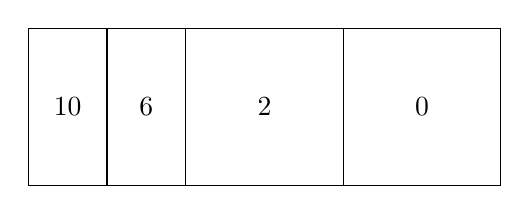
\begin{tikzpicture}

\node[ draw, rectangle, minimum width=1cm, minimum height=2cm, inner sep=0pt] (A2) at (-.5, 0) {10};
\node[ draw, rectangle, minimum width=1cm, minimum height=2cm, inner sep=0pt] (B2) at (.5 , 0) {6};
\node[ draw, rectangle, minimum width=2cm, minimum height=2cm, inner sep=0pt] (C2) at (2 , 0) {2};
\node[ draw, rectangle, minimum width=2cm, minimum height=2cm, inner sep=0pt] (D2) at (4, 0) {0};
\end{tikzpicture}
\]
In the second step we allocate the remaining part of $6$ and half of $2$ onto $b^e_2 = 4$ so $\omega^2 = (1/2, 0, 1/2, 1)$.
\[
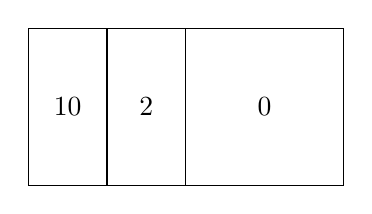
\begin{tikzpicture}
\node[ draw, rectangle, minimum width=1cm, minimum height=2cm, inner sep=0pt] (A2) at (-.5, 0 ) {10};
\node[ draw, rectangle, minimum width=1cm, minimum height=2cm, inner sep=0pt] (B2) at (.5 , 0) {2};
\node[ draw, rectangle, minimum width=2cm, minimum height=2cm, inner sep=0pt] (C2) at (2 , 0) {0};
\end{tikzpicture}
\]
Finally in the last step we allocate $1/10$ of $10$, all the remaining part of $2$ and $2/5$ of $0$ onto $b^e_3 = 2$ so $\omega^3 = (2/5, 0, 0, 3/5)$.
\[
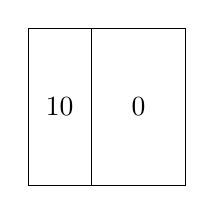
\begin{tikzpicture}
\node[ draw, rectangle, minimum width=.8cm, minimum height=2cm, inner sep=0pt] (A2) at (0, 0 ) {10};
\node[ draw, rectangle, minimum width=1.2cm, minimum height=2cm, inner sep=0pt] (B2) at (1 , 0) {0};

\end{tikzpicture}
\]


\end{example}

\begin{definition} The support of $M'_i$ denoted $\Supp(M'_i)$ is the set of all $1 \leq j \leq n$ such that $M'_{i, j} \neq 0$.
\end{definition}
\begin{lemma} {\label{support} } In our greedy allocation strategy, for every $i$,
\begin{enumerate}
\item The sequence $ \max Supp(M'_i)$ is non-decreasing in $i$.
\item If $ \min Supp(M'_i) < j < \max Supp(M'_i)$, then $\omega^k_{j} = 0$ for $k \geq i$.
\end{enumerate}
\end{lemma}
\begin{proof} b) follows directly from the construction of the greedy allocation strategy. For part a), we note that if $i < j$ and $\max \Supp(M'_i) > \max \Supp(M'_j)$, then by part b), we have either
\begin{itemize}
\item $\min \Supp(M'_i) < \max \Supp(M'_i)$ and $\min \Supp(M'_i) \geq \max Supp(M'_j)$.
\item $\min \Supp(M'_i) = \max \Supp(M'_i)$ and $\min \Supp (M'_i) > \max Supp(M'_j)$
\end{itemize} In either case this is a contradiction since $b^{e}_j \leq b^e_i$, $b^e_k$ is a convex combination of $c_r$ where $r$ ranges over the support of $M'_k$ for all $k$, $c_r$ is non-increasing, and $t$ is chosen to be minimal in the greedy allocation strategy.
\end{proof}
The following is a key Lemma that will be used repeatedly and demonstrates a lot of the power of the greedy allocation strategy.
\begin{lemma}\label{lemma_glue}
If our greedy allocation strategy completes at least $k$ steps, then for any integer $m \in [0, \omega_1 + \cdots + \omega_n]$,
\[
m = \omega^k_1 + \cdots + \omega^k_{I_{a^e, \omega^k} (m)}
\]
Moreover, for any $i$, the support of $M'_i$ lies completely in either $\{1, \cdots, I_{a^e, \omega^k} (m) \}$ or in $\{ I_{a^e, \omega^k} (m) + 1, \cdots , n \}$.
\end{lemma}
\begin{proof} We induct on the step in the greedy allocation strategy. It is obvious for step $0$. Suppose it holds for step $i - 1$. Then let $m \in [0, \omega^i_1 + \cdots + \omega^i_n]$ and let $t = \min \Supp(M'_i)$. If $I_{a^e, \omega^i} (m) <  t$, then we are done by induction. On the other hand suppose $I_{a^e, \omega^i} (m) \geq t$. By the construction of greedy allocation strategy $\omega^i_t < \omega^{i - 1}_t$  and $\omega^i_j = \omega^{i - 1}_j$ for $j < t$. So $I_{a^e, \omega^{i - 1}} \geq t$ and so by induction,
\[
m \geq \omega^{i - 1}_1 + \cdots + \omega^{i - 1}_t > \omega^{i }_1 + \cdots + \omega^{i}_t
\]
which implies $I_{a^e, \omega^i} (m) > t$. Let $t' = \max \Supp(M')$. By Lemma \ref{support}, $\omega^i_j = 0$ for $t < j < t'$. Therefore $I_{a^e, \omega^i} (m) \geq t'$. By the other part of Lemma \ref{support}, for $j \leq i$, $\max \Supp(M'_j) \leq \max \Supp(M'_i) \leq I_{a^e, \omega^i}(m)$ and so the support of $M'_j$ lies in $\{1, \cdots, I_{a^e, \omega^k} \}$. Using this we also obtain,
\[
I_{a^e, \omega^k} (m) = \omega^i_1 + \cdots + \omega^i_{I_{a^e, \omega^i} (m)} + \sum_{j = 1}^{i - 1} \sum_{k = 1}^{n} M'_{j, k} = (\omega^i_1 + \cdots + \omega^i_{I_{a^e, \omega^i}(m)} - m) + m + i - 1
\]
Therefore $ \omega^i_1 + \cdots + \omega^i_{I(m)} - m $ is an integer. But $ 0 \leq \omega^i_1 + \cdots + \omega^i_{I(m)} - m < 1$ so $m = \omega^i_1 + \cdots + \omega^i_{I(m)}$.
\end{proof}
\begin{definition} We let $\gamma(i)$ be the largest integer such that $a^o_{\gamma(i)} \geq b^o_i$ and $0$ if no such integer exists.
\end{definition}

Let us restate the definition of majorizing with parity in a form that will be more useful.
\begin{definition} A set non-negative integers $\{ \beta(i, j) \}_{i \in [0, \dim(b^o)], j \in [0, \dim(b^e)]}$ is a majorizer of $b$ if for all $i, j$, $\beta(i, j) \leq \gamma(i)$, $0 \leq i + j - \beta(i,j) \leq \dim(a^e)$ and
\[
\left ( \sum_{k = 1}^i b^o_k \right ) + \left ( \sum_{k = 1}^j b^e_k \right ) \leq \left ( \sum_{k = 1}^{\beta(i, j)} a^o_k \right ) + \left (\sum_{k = 1}^{ i + j - \beta(i, j) } a^e_k \right )
\]
\end{definition}
Observe that majorizing with parity is equivalant to a majorizer existing.
\begin{lemma} \label{major_suffix} Suppose that there exists a majorizer $\beta(i, j)$. Then for any $k \geq 0$, the sequence $a^o_{\dim(a^o) - k}, \cdots, a^o_{\dim(a^o)}$ majorizes $b^o_{\dim(b^o) - k}, \cdots, b^o_{\dim(b^o)}$
\end{lemma}
\begin{proof} Let $k \geq j \geq 0$. We have
\[
\gamma( \dim(b^o) - k) \geq \beta( \dim(b^o) - j, \dim(b^e) ) \geq \dim(b^o) - j
\]
\end{proof}




\begin{lemma} \label{increasing}
Suppose there exists a majorizer $\beta(i,j)$. Then there exists a majorizer $\beta'(i, j)$ such that
\[
\beta'(i, j) \leq \beta'(i + 1, j) \leq \beta'(i, j) + 1
\]
and
\[
\beta'(i, j) \leq \beta'(i, j + 1)
\]
for all $i, j$.
\end{lemma}
\begin{proof}
Let us assume that $\beta(i,j)$ is the majorizer which maximizes $ \left ( \sum_{k = 1}^{\beta(i, j)} a^o_k \right ) + \left (\sum_{k = 1}^{ i + j - \beta(i, j) } a^e_k \right )$ and then as a tiebreaker, maximizes $\beta(i, j)$. We first claim that $\beta(i, j)$ is non-decreasing. Suppose towards contradiction it is. Then there exists an $i, j$ such that $\beta(i, j) > \beta(i + 1, j)$ or $\beta(i, j) > \beta(i, j + 1)$. First assume the former is the case. Since $\beta(i, j)$ is a maximizer, we have $a^o_{\beta(i, j)} \geq a^e_{i + j - \beta(i, j) + 1}$. But then using the fact that $a^o$ and $a^e$ are non-increasing,
\[
\sum_{k = 1}^{\beta(i + 1, j ) } a^o_k + \sum_{k = 1}^{i + j + 1 - \beta(i + 1, j) } a^e_k \leq \sum_{k = 1}^{\beta(i, j)} b^o_k + \sum_{k = 1}^{i + j + 1 - \beta(i, j)} b^e_k
\]
which contradicts $\beta(i, j)$ being a maximizer. A similar analysis works for the case where $\beta'(i, j + 1) < \beta'(i, j)$


\medskip
We will now show by induction a required $\beta'(i, j)$ exists with the additional property that $\beta'(i,j) \leq \beta(i, j)$. We do this by induction on $i$. Since $\gamma(0) = 0$, $\beta(0, j) = \beta'(0, j) = 0$. Now given $\beta'(i, j)$ we let $\beta'(i + 1, j) = \beta'(i, j)$ if either $\beta'(i, j) = \gamma(i)$, or $a^e_{\beta'(i, j) + 1} < a^o_{i + j + 1 - \beta'(i, j)}$. Otherwise we let $\beta'(i + 1, j) = \beta'(i ,j ) + 1$. We need to verify that $\beta'(i + 1, j) \leq \beta(i + 1, j)$ and
\[
\left ( \sum_{k = 1}^{i + 1} b^o_k \right ) + \left ( \sum_{k = 1}^j b^e_k \right ) \leq \left ( \sum_{k = 1}^{\beta(i + 1, j)} a^o_k \right ) + \left (\sum_{k = 1}^{ i + j +1 - \beta(i + 1, j) } a^e_k \right )
\]
If the former is the case, then since $\beta(i + 1, j)$ is a maximizer and $\beta'(i, j) \leq \beta(i, j)$, $\beta'(i + 1, j) = \beta(i + 1, j)$ If the later is the case, then $\beta'(i, j) + 1 < \gamma(i) + 1 \leq \gamma(i + 1) + 1$, so $\beta'(i, j) + 1 \leq \gamma(i + 1)$. And
\begin{align*}
\left ( \sum_{k = 1}^{i + 1} b^o_k \right ) + \left ( \sum_{k = 1}^j b^e_k \right ) &\leq b^o_{i +1} + \left ( \sum_{k = 1}^{\beta(i, j)} a^o_k \right ) + \left (\sum_{k = 1}^{ i + j- \beta(i , j) } a^e_k \right )\\
& \leq \left ( \sum_{k = 1}^{\beta(i, j) + 1} a^o_k \right ) + \left (\sum_{k = 1}^{ i + j - \beta(i, j) } a^e_k \right )
\end{align*}
The fact that $\beta'(i, j) \leq \beta'(i, j + 1)$ follows from a simple induction on $i$.
\end{proof}
\begin{lemma} \label{no_abort} Suppose that there exists a majorizer $\beta(i, j)$, then the greedy allocation strategy does not abort.
\end{lemma}
\begin{proof} Recall that the greedy allocation strategy aborts iff there is some step $k$ in which we cannot find a $t$ for which $J_{a^e, \omega ^k } (t, t + 1) = b^e_k$. By the intermediate value theorem, this only happens in one of the following three cases
\begin{enumerate}
\item $|\omega^k|< 1$
\item $J_{a^e, \omega^k} (0, 1) < b^e_k$
\item $J_{a^e, \omega^k } ( |\omega^k| - 1, |\omega^k| ) > b^e_k$
\end{enumerate}
We will show none of these can happen. First we show $|\omega^k | \geq 1$. We have $|w^i| = \dim(b^e) - i$ and plugging in $i = 0, j = \dim(b^o)$ to the condition that $i + j \leq \gamma(i) + \dim(a^e)$ gives $\dim(b^o) \leq \dim(b^e)$.
\medskip
Next let us show that $J_{a^e, \omega^k} (0, 1) \geq b^e_k$. By lemma \ref{lemma_glue}, for every $j \leq k - 1$, the support of $M'_j$ is completely contained in either $\{1, \cdots , I_{a^e, \omega^k} ( 1) \}$ or $\{ I_{a^e, \omega^k} (1) +1, \cdots, \dim(b^e) \}$. If the later is the case then
\[
J_{a^e, \omega ^k} (0, 1) \geq \sum_{i} c_i M'_{j,i} = b^e_j \geq b^e_k
\]
If the former is the case for every $1\leq j \leq k - 1$, then
\[
J_{a^e, \omega^k} (0, 1) + \sum_{i = 1}^{k - 1} b^e_k = J_{a^e, \omega^k} (0, 1) + \sum_{j = 1}^{k - 1} \sum_i c_i M'_{j, i} = J_{a^e, \omega^1} (0, k) = \sum_{i = 1}^k a^e_i
\]
Rearranging give
\[
J_{a^e, \omega^k}(0, 1) = \sum_{i = 1}^{k} a^e_i - \sum_{i = 1}^{k - 1} b^e_i \geq b^e_k
\]
Finally we will show $J_{a^e, \omega^k } ( |\omega^k| - 1, |\omega^k| ) \leq b^e_k$. Note that $s := \dim(b^o) - \dim(a^o) = \dim(a^e) - \dim(b^e) \geq 0$. Let $r$ be the number of $M'_i$ whose support is contained in $\{1, \cdots, I_{a^e, \omega^k} (s) \}$. Let $t$ be the maximum non-negative integer such that $\beta(t, r) = (t + r) - (r + s) = t - s$. By Lemma \ref{increasing} we may assume $\beta(i, j) \leq \beta(i + 1, j) \leq \beta(i, j) + 1$ and $\beta(i, j) \leq \beta(i, j + 1)$. Note that $\beta(\dim(b^o), r) \leq \dim(a^o) =\dim(b^o) - s$ and $\beta(0, r) = r \geq -s$ so such a $t$ must exist by the discrete intemediate value theorem and Lemma \ref{no_abort}. By lemma \ref{lemma_glue},
\begin{align}
\sum_{i = 1}^{t} b^o_i + \sum_{i = 1}^{r} b^e_i & \leq \sum_{i = 1}^{ \beta(t, r) } a^o_i + \sum_{i = 1}^{s + r} a^e_s\\
& = \sum_{i = 1}^{\beta(t, r)} a^o_i + J_{a^e, \omega^k} (0, s) + \sum_{i = 1}^r b^e_i \\
&= \sum_{i = 1}^{\beta(t, r)} a^o_i + \sum_{i = 1}^{\dim(a^e)} a^e_i - J_{a^e, \omega^k} (s, |\omega^k| ) - \sum_{i = r + 1}^{k - 1} b^e_i\\
& = \sum_{i = 1}^{\dim(b^o)} b^o_i + \sum_{i = 1}^{\dim(b^o)} b^e_i - \sum_{i = \beta(t, r) + 1}^{\dim(a^o)} a^o_i - J_{a^e, \omega^k} (s, |\omega^k| ) - \sum_{i = r + 1}^{k - 1} b^e_i
\end{align}
Rearranging gives
\[
J_{a^e, \omega^k} (s, |\omega^k| ) \leq \left ( \sum_{i = r + 1}^{\dim (b^e)} b^e_i - \sum_{i = r + 1}^{k - 1} b^e_i \right ) + \left ( \sum_{i = t + 1}^{\dim(b^o)} b^o_i - \sum_{i = \beta(t, r) + 1}^{\dim(a^o)} a^o_i \right ) \leq \sum_{i = k }^{\dim(b^e)} b^e_i
\]
In the last step we are using Lemma \ref{major_suffix} to deduce that $ \sum_{i = t + 1}^{\dim(b^o)} b^o_i - \sum_{i = \beta(t, r) + 1}^{\dim(a^o)} a^o_i \leq 0$. Using this we get,
\[
J_{a^e, \omega^k} (|\omega^k| - 1, \omega^k )\leq \frac{1}{\dim(b^e) - k + 1} J_{a^e, \omega^k} (s, |\omega^k| ) \leq \frac{1}{\dim(b^e) - k + 1} \sum_{i = k }^{\dim(b^e)} b^e_i \leq b^e_k
\]
\end{proof}
\definition For $a, b \in \mathbb{Z}^n$, we say that a suballocation $M'$ of $a^e$ onto $b^e$ extends to an allocation if there exists an allocation of $(a^e, a^o)$ onto $(b^e, b^o)$ of the form
\[
\left[
\begin{array}{c|c}
M' & 0 \\
\hline
\multicolumn{2}{c}{M''}
\end{array}
\right]
\]
where $M''$ is a $\dim(b^o) \times n$ matrix.
\begin{lemma}\label{extends} Let $a, b \in \mathbb{Z}^n$. Suppose that $M'$ is a suballocation on $b^e$ and for $1 \leq i \leq \dim(a^e)$, let
\[
\omega_i = \sum_{j = 1}^{\dim(b^e)} M'_{j, i}
\]
Then $M'$ extends to an allocation if for every $1 \leq i \leq \dim(b^o)$, there exists an integer $\beta(i) \leq \gamma(i)$ such that
\[
a^o_1 + \cdots + a^o_{\beta(i)} + J_{a^e, w} (0, i - \beta(i)) \geq b^o_1 + \cdots + b^o_i
\]
\end{lemma}
\begin{proof}
We first note that by Lemma \ref{increasing}, we may assume $\beta(i)$ is non-decreasing. We will perform the following algorithm to construct a matrix $M'' \in \mathbb{R}^{\dim(b^o) \times n}$ such that
\[
\left[
\begin{array}{c|c}
M' & 0 \\
\hline
\multicolumn{2}{c}{M''}
\end{array}
\right]
\]
is an allocation of $(a^e, a^o)$ onto $(b^e, b^o)$ . We will initialize a matrix $ M'' = \boldsymbol{0} \in \mathbb{R}^{\dim(b^o) \times n}$. In the ith step of our algorithm, we will ensure that
\begin{enumerate}
\item $M''_{j, k} = 0$ for $j > i$.
\item $M \boldsymbol{1} = (1, \cdots, 1, 0, \cdots 0)$ where there are $i$ $1$'s.
\item $\boldsymbol{1}^T M \leq ( 1- \omega_1, \cdots, 1 - \omega_n)$
\item $M'' a \geq (b^o_1, \cdots b^o_i, 0 \cdots, 0)$
\end{enumerate}
We will keep track of a set $B$ and an integer $m$. We will aditionally maintain that $M''_{\ell,j} = 0$ for all $\ell$ and $j \in B$. $B$ is initialized to $ \emptyset$ and $m$ is initialized to $0$. In the ith step of our algorithm, we do the following. Start by adding all integers in the interval $ [\beta(i - 1) + 1, \beta(i) ]$ to $B$. Then if $B$ is non-empty, remove some $j \in B$ and set $M''_{i, j + \dim(a^e)} = 1$ and continue to step $i + 1$. Let us verify that $1-4$ are all satisifed. Clearly $1$ and $2$ are satisfied. Since $a^o_{j} \geq b^o_i$, we have $M'' a \geq ( b^o_1, \cdots, b^o_i, 0, \cdots, 0)$ so $4$ is satisifed. Since $M_{i, j}$ is the only non-zero entry in the $j$th column, we maintain $ \boldsymbol{1}^T M \leq (1 - \omega_1, \cdots, 1 - \omega_n)$ so $3$ is satisfied.
\medskip
If, on the other hand, $B$ is empty, we will set
\[
M_{i, j} = H_j (m, m + 1)
\]
for all $j \in [1, \dim(a^e)]$ and update $m$ to $m + 1$. If $\sum_{j = 1}^n M_{i, j} a_j \geq b_j$, then $1-4$ are satisfied and we continue to step $i + 1$. Otherwise initialize $v = \bf{0}$ and for $j = 1, \cdots, i - 1$, we do the following: let $t$ be the smallest positive real number such that either
\[
\sum_{k = 1}^n [(1 - t) M_{i, k} + v_k + (1 - |v|)t M_{j, k} ] a_k = b_i
\]
or
\[
\sum_{k = 1}^n [ t M_{i, k} + (1 - t + t|v| ) M_{j, k} ] a_k = b_j
\]
We note that such a $t$ must exist since when $t = 1$
\[
\sum_{k = 1}^n [ (1 - t) M_{i, j} + v_k + (1 - t + t|v|) M_{j k} ] a_k = \sum_{k = 1}^n \left ( \sum_{s = 1}^j \lambda_s M_{s, k} \right ) a_{j, k}
\]
for some $\lambda_1, \cdots, \lambda_j$ such that $\lambda_k \geq 0$ for all $k$, $\lambda_1 + \cdots + \lambda_j = 1$ and,
\[
\sum_{k = 1}^n \left ( \sum_{s = 1}^j \lambda_s M_{s, k} \right ) a_{j, k} \geq \sum_{s = 1}^j \lambda_s b^o_s \geq b^o_i
\]
After this, we update $M_{j, k}$ to $t M_{i, k} + (1 - t + t|v|) M_{j_k}$, update $M_{i, k}$ to $(1 - t) M_{i, k}$ and update $v_k$ to $ v_k + (1 - |v|) t M_{j, k}$.
\medskip
At the end of the process, update $M_{i, k}$ to $M_{i, k}+ v_k$. At this point either
\[
\sum_{k = 1}^n M_{i, k} a_k = b_i
\]
or
\[
\sum_{k = 1}^n M_{j, k} a_k = b_j
\]
for all $1 \leq j \leq i - 1$. If the first is the case $1-4$ are satisfied. If the second is the case then
\[
a^o_1 + \cdots + a^o_{\beta(i)} + J_{a^e, w}(0, i - \beta(i) ) = \sum_{j = 1}^i \sum_{k = 1}^n M_{j, k} a_k = b^o_1 + \cdots b^o_{i-1} + \sum_{k = 1}^n M_{i, k} a_k
\]
So
\[
\sum_{k = 1}^n M_{i, k} a_k \geq b^o_{i - 1}
\]
and $1-4$ are satisfied as well.
\end{proof}

\begin{lemma} \label{lemma_step} Suppose that $a$ majorizes $b$ with parity. Define $\beta(i)$ inductivly as follows. Let $\beta(0) = 0$, then for $i \geq 1$, 
\[
\beta(i) = \begin{cases} 1 + \beta(i - 1) & \beta(i - 1) < \gamma(i) \\  \beta(i - 1) & \beta(i - 1) = \gamma(i) \end{cases}
\]
Then there exists an integer $r$ such that $J_{a^e, w} (0, i - \beta(i) ) = (a^e_1 + \cdots a^e_r) - (b^e_1 + \cdots + b^e_{r - i + \beta(i)})$ and
\[
\left ( \sum_{k = 1}^{\beta(i)} a^o_{k} \right ) + \left ( \sum_{k = 1}^{r} a^e_k \right )  \geq  \left ( \sum_{k = 1}^i b^o_i \right ) + \left ( \sum_{k = 1}^{r - i + \beta(i) } b^e_k \right )
\]
\end{lemma}

\begin{proof} The fact that there exists an $r$ such that $J_{a^e, w} (0, i - \beta(i) ) = (a^e_1 + \cdots a^e_r) - (b^e_1 + \cdots + b^e_{r - i + \beta(i)})$ follows from Lemma \ref{lemma_glue}. For the second part we induct on $i$. Clearly it holds for $i = 0$. Now suppose it holds for $i - 1$. If $\beta(i) = 1 + \beta(i - 1)$, then since $\beta(i) \leq \gamma(i)$, $a^o_{\beta(i)} \geq b^o_i$ and so
\[
\left ( \sum_{k = 1}^{\beta(i)} a^o_{k} \right ) + \left ( \sum_{k = 1}^{r} a^e_k \right )  \geq a^o_{\beta(i) } + \left ( \sum_{k = 1}^{i - 1} b^o_i \right ) + \left ( \sum_{k = 1}^{r - i + \beta(i) } b^e_k \right )  \geq \left ( \sum_{k = 1}^i b^o_i \right ) + \left ( \sum_{k = 1}^{r - i + \beta(i) } b^e_k \right )
\]
Now suppose on the other hand that $\beta(i) = \beta(i - 1)$. In this case $\beta(i) = \gamma(i)$. Let $r'$ be the integer such that $J_{a^e, w} (0, i  - 1 - \beta(i) ) = (a^e_1 + \cdots a^e_{r'}) - (b^e_1 + \cdots + b^e_{r' - i + \beta(i)})$. If $J_{a^e, w} (i - \beta(i) - 1, i - \beta(i) ) \geq b^o_i$, then
\begin{align*}
\left ( \sum_{k = 1}^{\beta(i)} a^o_{k} \right ) + \left ( \sum_{k = 1}^{r} a^e_k \right )  
&=   \left ( \sum_{k = 1}^{\beta(i - 1)} a^o_{k} \right ) + \left ( \sum_{k = 1}^{r'} a^e_k \right )  + J_{a^e, w} (i - \beta(i) - 1, i - \beta(i) ) + \left ( \sum_{k = r' - i + \beta(i) }^{r - i + \beta(i) } b^e_k \right ) \\
& \geq  \left ( \sum_{k = 1}^i b^o_k \right ) + \left ( \sum_{k = 1}^{r - i + \beta(i) } b^e_k \right )
\end{align*}
So assume $J_{a^e, w} (i - \beta(i) - 1, i - \beta(i) ) < b^o_i$.
By assumption there exists an integer $s \leq \gamma(i)$ such that
\[
 \left ( \sum_{k = 1}^{s}  a^o_k  \right )  + \left ( \sum_{k = 1}^{r + \beta(i) - s}  a^e_k \right )  \geq  \left ( \sum_{k = 1}^i b^o_i \right ) + \left ( \sum_{k = 1}^{r - i + \beta(i) } b^e_k \right )
\]
but for $k > r$ and $t \leq \beta(i)$, by Lemma \ref{lemma_glue}, $a^e_k \leq J_{a^e, w} (i - \beta(i) - 1, i -\beta(i) ) < b^o_i \leq a^o_t$. Therefore,
\[
\left ( \sum_{k = 1}^{\beta(i)} a^o_{k} \right ) + \left ( \sum_{k = 1}^{r} a^e_k \right )  \geq  \left ( \sum_{k = 1}^{s}  a^o_k  \right )  + \left ( \sum_{k = 1}^{r + \beta(i) - s}  a^e_k \right )  \geq  \left ( \sum_{k = 1}^i b^o_i \right ) + \left ( \sum_{k = 1}^{r - i + \beta(i) } b^e_k \right )
\]

\end{proof}

\begin{lemma} \label{other_condition} Suppose there are at least $(i + j)$ elements from $a_1, \cdots, a_n$ that are either even or greater than or equal to $b^o_i$ and, letting $a'_1, \cdots, a'_{i + j}$ be the $(i + j)$ largest such elements (counted with multiplicity),
\[
\left ( \sum_{k = 1}^i b^o_k \right ) + \left ( \sum_{k = 1}^j b^e_k \right ) \leq \sum_{k = 1}^{i + j} a'_{k}
\]
Then there exists an allocation of $a$ onto $b$.
\end{lemma}
\begin{proof}
By lemma \ref{no_abort}, we can perform the greedy allocation of $a^e$. By lemma \ref{extends} it suffices to show there exists $\beta(i) \leq \gamma(i)$ such that
\[
\left ( \sum_{k = 1}^{\beta(i)} a^o_{k} \right ) + J_{a^e, w} (0, i - \beta(i) ) \geq b^o_1 + \cdots + b^o_i
\]
for all $i$. Take $\beta(i)$ as in Lemma \ref{lemma_step}. Then there exists an integer $r$ such that
\[
J_{a^e, w} (0, i - \beta(i) ) = (a^e_1 + \cdots a^e_r) - (b^e_1 + \cdots + b^e_{r - i + \beta(i)})
\]
and
\[
\left ( \sum_{k = 1}^{\beta(i)} a^o_{k} \right ) + J_{a^e, \omega} (0, i - \beta(i) ) = \left ( \sum_{k = 1}^{\beta(i)} a^o_{\beta(i)} \right ) + \left ( \sum_{k = 1}^{r} a^e_k \right ) - \left ( \sum_{k = 1}^{r - i + \beta(i) } b^e_k \right ) \geq \sum_{k = 1}^i b^o_i
\]
\end{proof}

We are finally ready to prove Theorem \ref{main}.

\begin{proof}[Proof of the if direction in Theorem \ref{main}] By Lemma \ref{rational_allocation_implies_theorem}, it suffices to show there exists a rational allocation of $a$ onto $b$. By Lemma \ref{allocation_implies_rational_allocation}, it suffices to show there exists an arbitrary allocation of $a$ onto $b$. By Lemma \ref{other_condition} this is true.
\end{proof}



\end{section}












\begin{section}{A Construction When $a$ Does Not Majorize $b$ With Parity} \label{sec4}
In this section we prove the only if direction of Theorem \ref{main}. So let $a_1, \cdots, a_n$ be a sequence that does not majorize $b_1, \cdots, b_n$ with parity. There exist indices $i_0, j_0$ such that either $\sum_{k = 1}^{i_0} b^o_k  + \sum_{k  = 1}^{j_0} b^e_k  >  \sum_{k  = 1}^{i_0 + j_0} a'_k$ or there are less than $i_0  + j_0$ elements in $a_1, \cdots, a_n$ that are either even or greater than or equal to $b^o_{i_0}$. 


\subsection{The General Case} We will start with focusing on the main case where the former holds, $i_0 > 0$, and $b_{i_0} > 1$.  The remaining cases are edge cases for which the same idea will work but we need to tweak the construction. 

\medskip

We may assume that 
\begin{equation}
 A' : =  \min \{ a'_1, \cdots, a'_{i_0 + j_0} \}  <  \min \{ b^o_{i_0}, b^e_{j_0} \} \label{assumption}
\end{equation}
as otherwise we could find a smaller pair $(i_0, j_0)$.

\begin{subsection}{The Construction of $G$}
 We will construct a graph $G$ using a parameter $M$ which, for $M$ sufficiently large, will satisfy $w_{a_1}(G) \cdots w_{a_n}(G) < w_{b_1}{G} \cdots w_{b_n} (G)$. $G$ will have two components $H$ and $K$. $H$ will be constructed out of $b^o_{i_0} + 1$ parts, $H_0, \cdots, H_{b^o_{i_0}}$ where $|H_0| = |H_{b^o_{i_0}}| = M^3$ and $|H_1| = |H_2| = \cdots = |H_{b^o_{i_0} - 1}| = M$. For $i \in [1, b^o_{i_0} - 1]$, $H_i$ and $H_{i + 1}$ will form a complete bipartite graph, each vertex in $H_1$ will be adjacent to $M^2$ unique vertices in $H_0$ and each vertex in $H_{b^o_{i_0} - 1}$ will be adjacent to $M^2$ unique vertices in $H_{b^o_{i_0}}$.  $K$ will be any $M^{1 - \vep}$ regular graph on $M^{3 + A' \vep}$ vertices where $\vep < 1/(1 + b_{i_0} - A')$ is a sufficiently small constant.  
\end{subsection}
\[
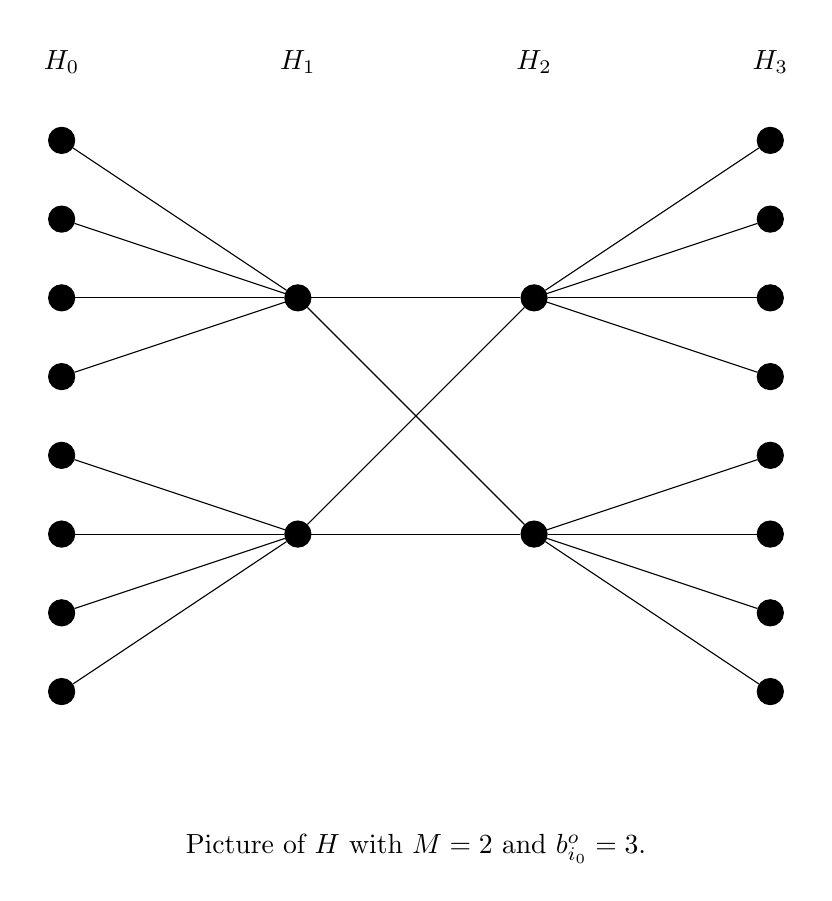
\begin{tikzpicture}
\tikzset{
  every arrow/.style={line width=1.5pt},
  >=stealth
}
\node[circle, fill = black, draw] (A1) at (0, 0){};
\node[circle, fill = black, draw] (A2) at (0, 1){};
\node[circle, fill = black, draw] (A3) at (0, 2){};
\node[circle, fill = black, draw] (A4) at (0, 3){};
\node[circle, fill = black, draw] (A5) at (0, 4){};
\node[circle, fill = black, draw] (A6) at (0, 5){};
\node[circle, fill = black, draw] (A7) at (0, 6){};
\node[circle, fill = black, draw] (A8) at (0, 7){};

\node[circle, fill = black, draw] (B1) at (3, 2){};
\node[circle, fill = black, draw] (B2) at (3, 5){};

\node[circle, fill = black, draw] (C1) at (6, 2){};
\node[circle, fill = black, draw] (C2) at (6, 5){};



\node[circle, fill = black, draw] (D1) at (9, 0){};
\node[circle, fill = black, draw] (D2) at (9, 1){};
\node[circle, fill = black, draw] (D3) at (9, 2){};
\node[circle, fill = black, draw] (D4) at (9, 3){};
\node[circle, fill = black, draw] (D5) at (9, 4){};
\node[circle, fill = black, draw] (D6) at (9, 5){};
\node[circle, fill = black, draw] (D7) at (9, 6){};
\node[circle, fill = black, draw] (D8) at (9, 7){};

\node[circle] (H0) at (0, 8){$H_0$};
\node[circle] (H1) at (3, 8){$H_1$};
\node[circle] (H2) at (6, 8){$H_2$};
\node[circle] (H3) at (9, 8){$H_3$};

\path (A1) edge (B1);
\path (A2) edge (B1);
\path (A3) edge (B1);
\path (A4) edge (B1);

\path (A5) edge (B2);
\path (A6) edge (B2);
\path (A7) edge (B2);
\path (A8) edge (B2);

\path (B1) edge (C1);
\path (B1) edge (C2);
\path (B2) edge (C1);
\path (B2) edge (C2);


\path (D1) edge (C1);
\path (D2) edge (C1);
\path (D3) edge (C1);
\path (D4) edge (C1);

\path (D5) edge (C2);
\path (D6) edge (C2);
\path (D7) edge (C2);
\path (D8) edge (C2);



\node[align = flush center, text width = 8cm] (Label) at (4.5, -2)
{
Picture of $H$ with $M = 2$ and $b^o_{i_0} = 3$.
};



\end{tikzpicture}
\]

\begin{lemma} \label{Hbound} Let $k$ be a non-negative integer and let 
\[
f(k) = \begin{cases}     M^{2 + k} &  k < b^o_{i_0}, k \equiv 1 \pmod 2 \\ M^{3 + k} & \text{else} \end{cases}
\]
then
\[
f(k)   \leq w_{k}(H)   \leq w_k(P_{b^o_{i_0} })  f(k)
\]







\end{lemma}
\begin{proof}
A walk of length $k$ in $H$ naturally projects down to a walk in $P_{b^o_{i_0}} = (0, \cdots b)$, by $\pi(p)_i$ is the index $j$ for which $p_i \in H_j$. Let us compute $|\pi^{-1}(p)|$. If $p_0 \in \{0, b^o_{i_0} \}$, then there are $M^3$ choices for $\pi^{-1}(p_0)$ and otherwise there are $M$ choices. Then for $i \geq 1$, there are $M^2$ choices for $\pi^{-1}(p_i)$ if $i \in \{0, b^o_{i_0}\}$, there is $1$ choice for $\pi^{-1}(p)$ if $p_{i - 1} \in \{0, b^o_{i_0}\}$, and there are $M$ choices otherwise. Putting this together we obtain, 
\[
|\pi^{-1} (p) | = M^{ k + 1 + \chi_{p_0  \in \{0, b^o_{i_0}\} } + \chi_{p_k \in \{0, b^o_{i_0}\} } }
\]  
Then the lemma follows from the fact that there exists a path $p$ of length $k$ such that $p_{0} \in \{0, b^o_{i_0} \}$ and $p_{k} \in \{ 0, b^o_{i_0} \}$ iff $k$ is even or $k$ is odd and greather than or equal to $b^o_{i_0}$.
\end{proof}


\begin{lemma} \label{weight_bound} Let $k$ be a non-negative integer. Then,
\[
w_k(G) = \begin{cases} \Theta(M^{3 + k} )  & k \equiv 0 \pmod 2,  k \geq A' \text{ OR }  k \equiv 1 \pmod 2,  k \geq b^o_{i_0} \\   
\Theta(M^{3 + A' \vep + (1 - \vep) k } )  &   \text{ else } 
\end{cases}
\]
\end{lemma}
\begin{proof} Using the $f(k)$ in Lemma \ref{Hbound},
\begin{align*}
w_k(G) & = \Theta ( \max \{ w_k(H), w_k(K) \} )\\
 & = \Theta ( \max \{  f(k),  M^{3 + A' \vep + (1 - \vep) k } \} )\\
& =  \begin{cases} \Theta(M^{3 + k} )  & k \equiv 0 \pmod 2,  k \geq A' \text{ OR }  k \equiv 1 \pmod 2,  k \geq b^o_{i_0} \\   
\Theta(M^{3 + A' \vep + (1 - \vep) k } )  &   \text{ else } 
\end{cases}
\end{align*}

\end{proof}
We can now prove the only direction in Theorem \ref{main} in this general case.
\begin{proof} [Proof of the only direction of Theorem \ref{main} in the general case ] Let $S := \sum_{k = 1}^n a_k = \sum_{k = 1}^n b_k$. Let $\hat{a}_1, \cdots, \hat{a}_{n - i_0 - j_0}$ be the elements in $a$ not appearing in $a'_1, \cdots, a'_{i_0 + j_0}$. By assumption \ref{assumption} each element in $\{\hat{a}_1, \cdots, \hat{a}_{n - i_0 - j_0} \}$ is either even and less than or equal to $A'$ or odd and less than $b_{i_0}$. By Lemma \ref{weight_bound},
\begin{align*}
w_{b_1}(G) \cdots w_{b_n}(G) & \geq \Theta \left ( \left ( \prod_{k = 1}^{i_0} M^{3 + b^o_k}  \right )  \left ( \prod_{k = 1}^{j_0} M^{3 + b^e_k} \right ) \left ( \prod_{k = i_0 + 1}^{\dim(b^o)}  M^{3 + A' \vep + (1 - \vep) b^o_k } \right ) \left ( \prod_{k = j_0 + 1}^{\dim(b^e) }M^{3 + A' \vep + (1 - \vep) b^e_k}  \right ) \right )\\
&=  \Theta \left ( M^{3n + (1 - \vep) S  +  (n - i_0 - j_0) A' \vep +  \left ( \sum_{k = 1}^{i_0}  b^o_k  + \sum_{k = 1}^{j_0} b^e_k \right ) \vep } \right ) \\
& \gg  \Theta \left ( M^{3n + (1 - \vep) S + (n - i_0 - j_0) A' \vep +  \left ( \sum_{k = 1}^{i_0 + j_0} a'_k \right ) \vep  } \right )\\
& = \Theta \left (  \left ( \prod_{k = 1}^{i_0 + j_0}  M^{3 + a'_{k} } \right ) \left ( \prod_{k = 1}^{n - i_0 - j_0} M^{3 + A' \vep + (1 - \vep) \hat{a}_k } \right ) \right ) \\
& = w_{a_1}(G) \cdots w_{a_n}(G)
\end{align*}
\end{proof}
In the above $\Theta$ is with respect to $M$.
\subsection{The Edge Cases} We will now describe how to change the construction of $G$ in the following three remaining cases
\begin{enumerate}
\item $i_0 = 0$
\item $b_{i_0} = 1$
\item  There are less than $i_0  + j_0$ elements in $a_1, \cdots, a_n$ that are either even or greater than or equal to $b^o_{i_0}$. 
\end{enumerate}
If 1 holds, instead of having $b^o_{i_0}$ parts, then we take $H$ to have at least $\max \{ b^o_1 , a^o_1 \} + 3$ parts (or an arbitrary number of parts if $a$ and $b$ have no odd components). If 2 holds, we replace $H$ with an $M$ regular graph with $M^3$ vertices. If 3 holds then we let $G = H$ instead of $G = H \sqcup K$. Note that 1 and 3 may hold simultaneously in which case we both take $H$ to have at least $\max \{b^o_1, a^o_1 \} + 3$ components and let $G = H$. In all these cases, the same computation that we did in the general case will apply.
\end{section}

\begin{thebibliography}{99}
\bibitem{BR} Blekherman, Raymond, Proof of the Erd\H{o}s-Simonovits conjecture on walks, Graphs and Combinatorics 39 (3) 53
\bibitem{BlR} George Blakley and Prabir Roy. H\"older type inequality for symmetric matrices with nonnegative entries. Proceedings of the American Mathematical Society, 16:1244-1245, 1965.
\bibitem{ES} P. Erd\H{o}s and M. Simonovits. Compactness results in extremal graph theory. Combinatorica, 2(3):275-283, 1982.
\bibitem{HK} R. Hemmecke, S. Kosub, E. mayr, H. T\"aubig, J. Weihmann. Inequalities for the Number of Walks in graphs. Algorithmica, 66, 804-828, (2013).
\bibitem{DG} A. Dress and I. Gutman. The number of walks in a graph. Applied Mathematics Letters, 16(5): 797-801, July 2003.
\bibitem{LM} J. Lagarias, J. Mazor, L. Shepp, B. McKay. An inequality for walks in a graph. IAM Review, 25(3):403, July 1983.
\bibitem{BR2} Blekherman, Grigoriy, and Annie Raymond. "A Path Forward: Tropicalization in Extremal Combinatorics." Advances in Mathematics, vol. 407, 2022, article 108561.
\end{thebibliography}
\end{document}

